
\documentclass[11pt]{article}
\usepackage{amsmath, amssymb, amsthm}
\usepackage{geometry}
\usepackage{graphicx}
\geometry{margin=1in}
\title{Foundations of Machine Learning -- Lecture 6 Notes}
\author{}
\date{}
\setlength{\parindent}{0pt}

\begin{document}
\maketitle

\section*{Dimensionality Reduction}
We care about this to overcome the curse of dimensionality, and to better compress our data.
It also leads to simpler data visualization and denoising.

\begin{figure}[h!]
	\centering
	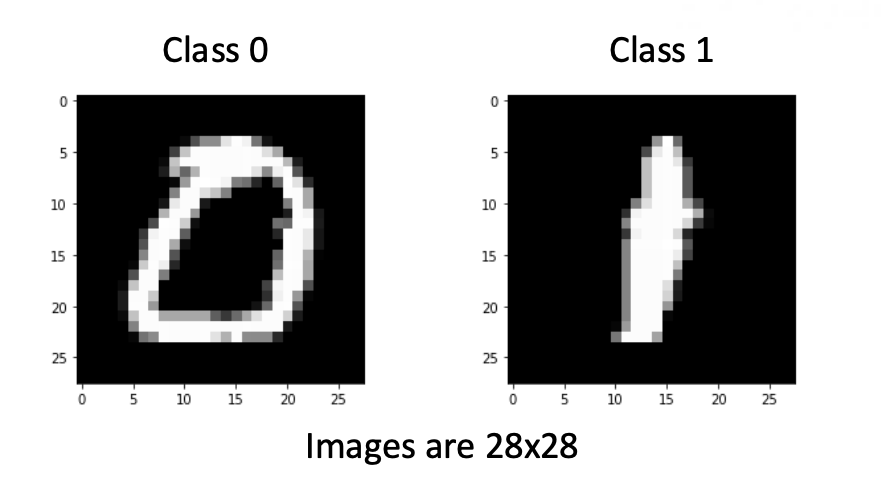
\includegraphics[width=0.6\textwidth]{../imgs/MNIST.png}
	\caption{MNIST handwritten classification dataset}
\end{figure}

We can vectorize the dataset:
\[
	x^{(i)} \in \mathbb{R}^{784}
	\quad
	y^{(i)} \in {0,1}
\]

One option to reduce dims is to use principle components, and only track 2 features of the images, one being how line-like it is and another for how curved it is.

\begin{figure}[h!]
	\centering
	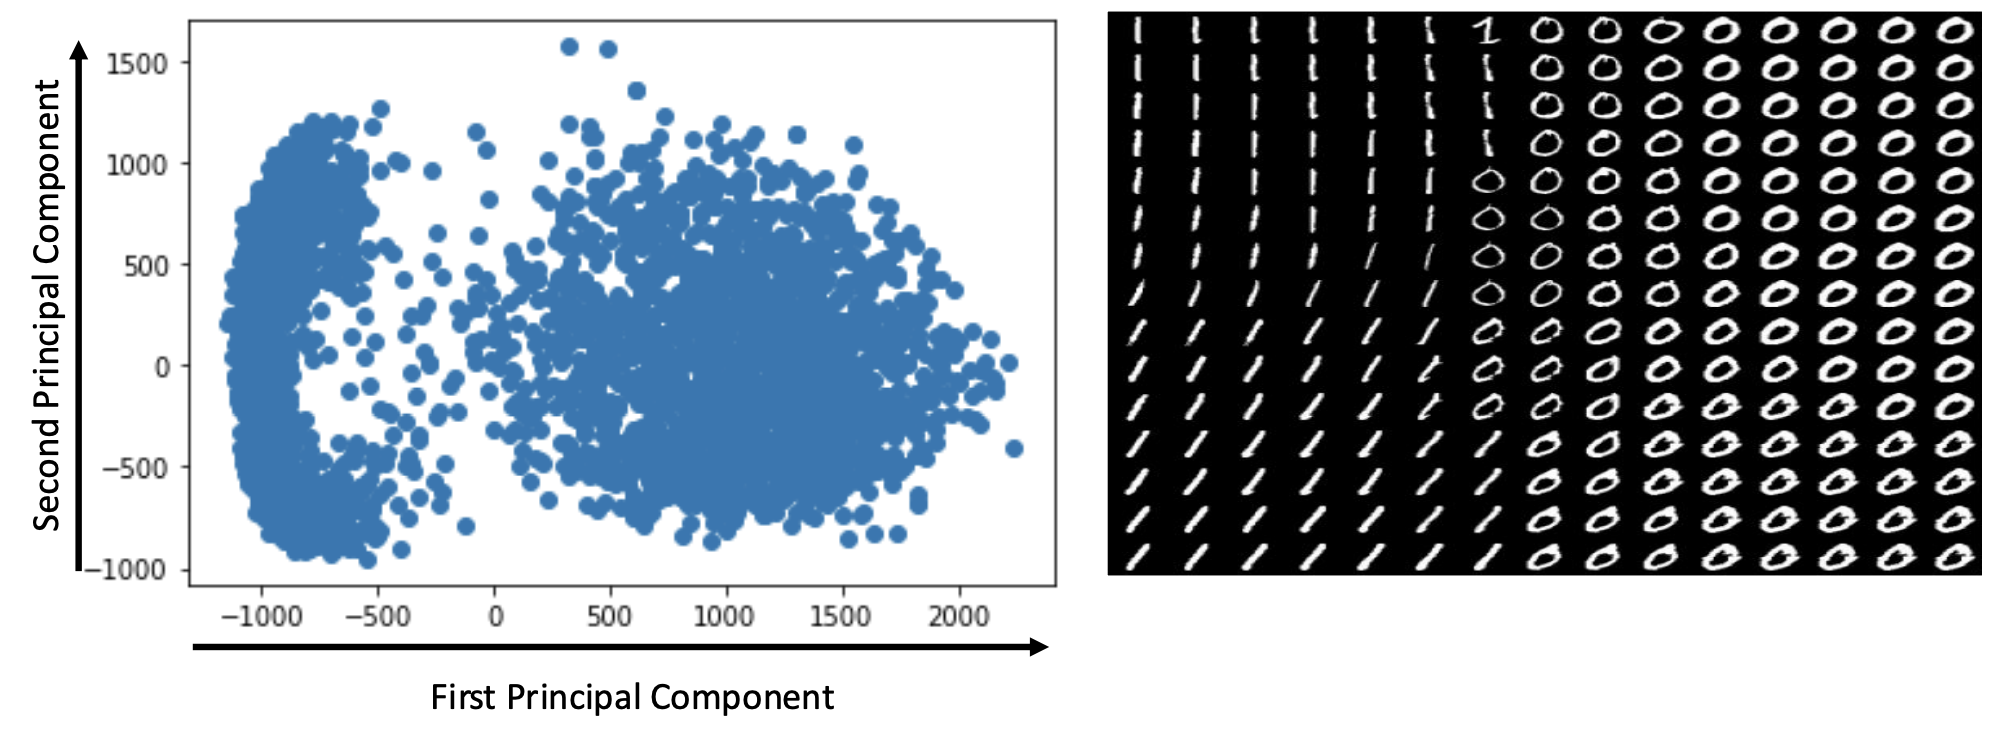
\includegraphics[width=0.6\textwidth]{../imgs/pcomps.png}
	\caption{MNIST handwritten classification dataset}
\end{figure}

\pagebreak

Whatever method we choose the main goal is for our reduced data to preserve as much information as possible.
\[
	f: \mathbb{R}^d \rightarrow \mathbb{R}^k \quad k<d
\]
\[
	x \in \mathbb{R}^d
\]
\[
	z = f(x) \in \mathbb{R}^k
\]

We may want to be able to recover x from z as closely as possible.

\subsection*{Maximizing Variance}

Find $w$ such that it maximizes the variance of the projected data

We have data
\[
	x = \{x_1, x_2,\dots, x_N\in \mathbb{R}^d\}
\]

Our reduced data is
\[
	\left\{ z_i =w^Tx_i \right\}_{i=1}^{N}
\]


Let’s first calculate the mean of the reduced data:
\[
	\bar{z} = \frac{1}{N} \sum_{i=1}^{N} z_i
	= \frac{1}{N} \sum_{i=1}^{N} \mathbf{w}^T \mathbf{x}_i
	= \mathbf{w}^T \left( \frac{1}{N} \sum_{i=1}^{N} \mathbf{x}_i \right)
	= \mathbf{w}^T \bar{\mathbf{x}}
\]
Then the variance of the reduced data is:
\[
	\mathrm{var} = \frac{1}{N} \sum_{i=1}^{N} (z_i - \bar{z})^2
	= \frac{1}{N} \sum_{i=1}^{N} \left( \mathbf{w}^T (\mathbf{x}_i - \bar{\mathbf{x}}) \right)^2
\]

\[
	\text{var} = \frac{1}{N} \sum_{i=1}^{N} \left(w^T(x_i - \bar{x})\right)^2
	= \frac{1}{N} \sum_{i=1}^{N} w^T(x_i - \bar{x})(x_i - \bar{x})^T w
\]

\[
	= w^T \left( \frac{1}{N} \sum_{i=1}^{N} (x_i - \bar{x})(x_i - \bar{x})^T \right) w
	= w^T S w
\]

\[
	\text{Therefore maximizing the variance can be written as:}
\]

\[
	\max_{w} \quad w^T S w \quad \text{s.t.} \quad w^T w = 1
\]
High variance: Data points are well spread and captures meaningful differences between samples
Low variance: Almost constant and carries little distinction across data

\medskip

We set the constraint to be $w^tw = 1$ so that our w corresponds to an actual direction change instead of just bumping magnitude.

Any solution to this must satisfy:

\[
	S w = \lambda w, \qquad w^T w = 1
\]

\medskip

But we want to find the eigenvector that maximizes $w^T S w$

\pagebreak

Some characteristics of eigenvectors:
\begin{itemize}
	\item $\|v_i\| = 1$
	\item $v_i^T v_j = 0,\;\; \forall i \ne j$ \quad (orthogonal)
\end{itemize}

\medskip
Covariance matrix $S$ is real and symmetric (PSD), so it can be uniquely decomposed as:

\[
	S = \sum_i \lambda_i v_i v_i^T
\]

Multiply both sides by eigenvector $v_k$:

\[
	v_k^T S v_k = \lambda_k
\]

\bigskip

Therefore, $w$ should be the first eigenvector (largest eigenvalue) of $S$.


\subsection*{Minimizing Reconstruction Error}

In order to reconstruct from $z \rightarrow x$ we see the following:

\[
	\hat{x} = w w^T x
\]

Now we can write the reconstruction error as:

\begin{align}
	\frac{1}{N} \sum_{i=1}^{N} \left\| \hat{x}^{(i)} - x^{(i)} \right\|^2
	 & = \frac{1}{N} \sum_{i=1}^{N} \left\| ww^T x^{(i)} - x^{(i)} \right\|^2
\end{align}

This is equivalent to maximizing the variance! 

\end{document}

